Here we introduce the Rolling Entropy Sampler (RES), a sampler that commits tokens neither at acceptance nor at the end of the block.
The core mechanism is simple: instead of waiting for the entire block to converge, RES encodes any sufficiently long contiguous prefix of accepted tokens, appends it to the KV cache, and refills the freed slots with fresh noise.
Positions outside the committed prefix, accepted or not, remain free to change.
Figure~\ref{fig:algorithm-concept} illustrates the method.
\begin{figure}[tbp]
\centering
\begin{tikzpicture}[x=0.36cm, y=0.36cm]

\definecolor{cclean}{HTML}{FFFFFF}
\definecolor{ccleanedge}{HTML}{B4B4A9}
\definecolor{cwinedge}{HTML}{0F6E56}
\definecolor{cwinfill}{HTML}{9FE1CB}
\definecolor{cnoise}{HTML}{D3D1C7}
\definecolor{cnoiseedge}{HTML}{888780}
\definecolor{cframe}{HTML}{2B5E94}
\definecolor{camber}{HTML}{E8A13C}
\definecolor{camberedge}{HTML}{A96A0B}
\definecolor{mempty}{HTML}{F5F4EF}
\definecolor{memptyedge}{HTML}{C9C7BE}

\newcommand{\cellclean}[3]{%
  \fill[cclean, draw=ccleanedge, line width=0.4pt, rounded corners=1pt] (#1, #2) rectangle ++(0.9, 1);
  \node[font=\scriptsize\ttfamily, inner sep=0pt, text=black] at (#1+0.45, #2+0.5) {#3};}
\newcommand{\cellwin}[4]{%
  \fill[cwinfill!#3, draw=cwinedge, line width=0.4pt, rounded corners=1pt] (#1, #2) rectangle ++(0.9, 1);
  \node[font=\scriptsize\ttfamily, inner sep=0pt, text=black] at (#1+0.45, #2+0.5) {#4};}
\newcommand{\cellnoise}[3]{%
  \fill[cnoise, draw=cnoiseedge, line width=0.4pt, rounded corners=1pt] (#1, #2) rectangle ++(0.9, 1);
  \node[font=\scriptsize\ttfamily, inner sep=0pt, text=cnoiseedge] at (#1+0.45, #2+0.5) {#3};}
\newcommand{\cellamber}[3]{%
  \fill[camber!45, draw=camberedge, line width=0.6pt, rounded corners=1pt] (#1, #2) rectangle ++(0.9, 1);
  \node[font=\scriptsize\ttfamily, inner sep=0pt, text=black] at (#1+0.45, #2+0.5) {#3};}
\newcommand{\acceptmark}[2]{\draw[camberedge, line width=1.1pt, rounded corners=1pt] (#1+0.03, #2+0.03) rectangle ++(0.84, 0.94);}
\newcommand{\acceptdot}[2]{\fill[camberedge] (#1+0.45, #2+0.17) circle (0.12);}
\newcommand{\passframe}[2]{%
  \draw[cframe, line width=1.1pt, rounded corners=2pt, dash pattern=on 4pt off 2pt]
    (#1-0.15, #2-0.25) rectangle (#1+10.05, #2+1.25);}
\newcommand{\seqbracket}[4]{%
  \draw[line width=0.3pt] (#1, #3-0.55) -- (#1, #3-0.90) -- (#2+0.9, #3-0.90) -- (#2+0.9, #3-0.55);
  \node[font=\tiny, anchor=north, inner sep=1.5pt] at ({(#1+#2+0.9)/2}, #3-0.90) {#4};}

\newcommand{\maskpanel}[5]{%
\begin{scope}[shift={(#4cm,#5cm)}, x=0.19cm, y=0.19cm]
  \foreach \q in {#1,...,#2}{%
    \foreach \k in {#1,...,#2}{%
      \pgfmathtruncatemacro{\ii}{\k-#1}%
      \pgfmathtruncatemacro{\jj}{\q-#1}%
      \ifnum\q>#3\relax
        \ifnum\k>#3\relax
          \fill[cwinfill!65, draw=cwinedge, line width=0.25pt, rounded corners=0.4pt] (\ii,-\jj) rectangle ++(0.88,-0.88);
        \else
          \fill[camber!20, draw=camberedge, line width=0.25pt, rounded corners=0.4pt] (\ii,-\jj) rectangle ++(0.88,-0.88);
        \fi
      \else
        \ifnum\k>\q\relax
          \fill[mempty, draw=memptyedge, line width=0.25pt, rounded corners=0.4pt] (\ii,-\jj) rectangle ++(0.88,-0.88);
        \else
          \fill[camber!55, draw=camberedge, line width=0.25pt, rounded corners=0.4pt] (\ii,-\jj) rectangle ++(0.88,-0.88);
        \fi
      \fi}}%
  \pgfmathtruncatemacro{\cc}{#3-#1+1}%
  \pgfmathtruncatemacro{\nn}{#2-#1+1}%
  \ifnum\cc>0\relax
    \draw[dashed, line width=0.4pt] (\cc-0.06, 0.5) -- (\cc-0.06, -\nn-0.1);
    \draw[dashed, line width=0.4pt] (-0.5, -\cc+0.06) -- (\nn+0.1, -\cc+0.06);
    \draw[camberedge, line width=0.8pt, rounded corners=0.6pt] (-0.06, 0.06) rectangle (\cc-0.12, -\cc+0.12);
  \fi
\end{scope}}
\newcommand{\maskbrackets}[4]{%
\begin{scope}[shift={(#3cm,#4cm)}, x=0.19cm, y=0.19cm]
  \ifnum#1>0\relax
    \draw[line width=0.3pt] (0,-#2-0.5) -- (0,-#2-0.9) -- (#1-0.12,-#2-0.9) -- (#1-0.12,-#2-0.5);
    \node[font=\tiny, anchor=north, inner sep=1.5pt] at (#1/2-0.06, -#2-0.9) {prefix};
  \fi
  \draw[line width=0.3pt] (#1,-#2-0.5) -- (#1,-#2-0.9) -- (#2-0.12,-#2-0.9) -- (#2-0.12,-#2-0.5);
  \node[font=\tiny, anchor=north, inner sep=1.5pt] at ({(#1+#2)/2-0.06}, -#2-0.9) {window};
\end{scope}}

\newcommand{\keyencoded}{\begin{tikzpicture}[baseline=-0.5ex, x=0.36cm, y=0.36cm]
  \fill[cclean, draw=ccleanedge, line width=0.4pt, rounded corners=1pt] (0,-0.5) rectangle ++(0.9,1);
\end{tikzpicture}}
\newcommand{\keyaccepted}{
\begin{tikzpicture}[baseline=-0.5ex, x=0.36cm, y=0.36cm]
  \fill[cwinfill!30, draw=cwinedge, line width=0.4pt, rounded corners=1pt] (0,-0.5) rectangle ++(0.9,1);
  \draw[camberedge, line width=1.1pt, rounded corners=1pt] (0.03,-0.47) rectangle ++(0.84,0.94);
\end{tikzpicture}}
\newcommand{\keywaiting}{
\begin{tikzpicture}[baseline=-0.5ex, x=0.36cm, y=0.36cm]
  \fill[cwinfill!30, draw=cwinedge, line width=0.4pt, rounded corners=1pt] (0,-0.5) rectangle ++(0.9,1);
  \fill[camberedge] (0.45,-0.33) circle (0.12);
\end{tikzpicture}}
\newcommand{\keyprefix}{
\begin{tikzpicture}[baseline=-0.5ex, x=0.36cm, y=0.36cm]
  \fill[camber!45, draw=camberedge, line width=0.6pt, rounded corners=1pt] (0,-0.5) rectangle ++(0.9,1);
\end{tikzpicture}}
\newcommand{\keynoise}{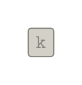
\begin{tikzpicture}[baseline=-0.5ex, x=0.36cm, y=0.36cm]
  \fill[cnoise, draw=cnoiseedge, line width=0.4pt, rounded corners=1pt] (0,-0.5) rectangle ++(0.9,1);
  \node[font=\scriptsize\ttfamily, inner sep=0pt, text=cnoiseedge] at (0.45,0) {k};
\end{tikzpicture}}
\newcommand{\keymcausal}{
\begin{tikzpicture}[baseline=-0.5ex, x=0.36cm, y=0.36cm]
  \fill[camber!55, draw=camberedge, line width=0.4pt, rounded corners=1pt] (0,-0.5) rectangle ++(0.9,1);
\end{tikzpicture}}
\newcommand{\keymcross}{
\begin{tikzpicture}[baseline=-0.5ex, x=0.36cm, y=0.36cm]
  \fill[camber!20, draw=camberedge, line width=0.4pt, rounded corners=1pt] (0,-0.5) rectangle ++(0.9,1);
\end{tikzpicture}}
\newcommand{\keymbidi}{
\begin{tikzpicture}[baseline=-0.5ex, x=0.36cm, y=0.36cm]
  \fill[cwinfill!65, draw=cwinedge, line width=0.4pt, rounded corners=1pt] (0,-0.5) rectangle ++(0.9,1);
\end{tikzpicture}}
\newcommand{\keymempty}{
\begin{tikzpicture}[baseline=-0.5ex, x=0.36cm, y=0.36cm]
  \fill[mempty, draw=memptyedge, line width=0.4pt, rounded corners=1pt] (0,-0.5) rectangle ++(0.9,1);
\end{tikzpicture}}

\node[anchor=east, font=\small\bfseries] at (-0.60, 0.50) {step $t$};
\cellclean{0}{0}{t}
\cellclean{1}{0}{h}
\cellclean{2}{0}{e}
\cellclean{3}{0}{}
\cellclean{4}{0}{c}
\cellclean{5}{0}{a}
\cellclean{6}{0}{t}
\cellclean{7}{0}{}
\cellwin{8}{0}{30}{m}
\cellwin{9}{0}{30}{e}
\cellwin{10}{0}{55}{r}
\cellwin{11}{0}{30}{w}
\cellwin{12}{0}{70}{s}
\cellwin{13}{0}{90}{}
\cellwin{14}{0}{100}{q}
\cellwin{15}{0}{100}{7}
\cellwin{16}{0}{100}{x}
\cellwin{17}{0}{100}{v}
\cellnoise{18}{0}{9}
\cellnoise{19}{0}{k}
\cellnoise{20}{0}{z}
\cellnoise{21}{0}{3}
\cellnoise{22}{0}{b}
\cellnoise{23}{0}{5}
\acceptmark{8}{0}
\acceptmark{9}{0}
\acceptmark{11}{0}
\passframe{8}{0}
\seqbracket{8}{17}{0}{10 positions per pass}
\maskpanel{8}{17}{7}{9.25}{1.13}

\node[font=\scriptsize, anchor=south, text=ccleanedge!60!black] at (3.95, 1.32) {KV cache};
\node[cframe, font=\scriptsize, anchor=south] at (12.95, 1.32) {processed this pass};
\node[cnoiseedge, font=\scriptsize, anchor=south] at (20.95, 1.32) {not yet admitted};
\node[font=\scriptsize, anchor=south] at (10.20cm, 1.57cm) {attention mask};
\node[font=\tiny, anchor=south] at (10.20cm, 1.19cm) {keys $\rightarrow$};
\node[font=\tiny, rotate=90, anchor=south] at (9.09cm, 0.18cm) {queries};

\node[anchor=east, font=\small\bfseries] at (-0.60, -6.50) {step $t{+}1$};
\cellclean{0}{-7.00}{t}
\cellclean{1}{-7.00}{h}
\cellclean{2}{-7.00}{e}
\cellclean{3}{-7.00}{}
\cellclean{4}{-7.00}{c}
\cellclean{5}{-7.00}{a}
\cellclean{6}{-7.00}{t}
\cellclean{7}{-7.00}{}
\cellamber{8}{-7.00}{m}
\cellamber{9}{-7.00}{e}
\cellwin{10}{-7.00}{30}{o}
\cellwin{11}{-7.00}{30}{w}
\cellwin{12}{-7.00}{30}{s}
\cellwin{13}{-7.00}{30}{}
\cellwin{14}{-7.00}{55}{l}
\cellwin{15}{-7.00}{55}{o}
\cellwin{16}{-7.00}{70}{u}
\cellwin{17}{-7.00}{70}{d}
\cellnoise{18}{-7.00}{9}
\cellnoise{19}{-7.00}{k}
\cellnoise{20}{-7.00}{z}
\cellnoise{21}{-7.00}{3}
\cellnoise{22}{-7.00}{b}
\cellnoise{23}{-7.00}{5}
\acceptmark{10}{-7.00}
\acceptdot{11}{-7.00}
\acceptmark{12}{-7.00}
\acceptmark{13}{-7.00}
\passframe{8}{-7.00}
\maskpanel{8}{17}{9}{9.25}{-1.39}

\node[anchor=east, font=\small\bfseries] at (-0.60, -13.50) {step $t{+}2$};
\cellclean{0}{-14.00}{t}
\cellclean{1}{-14.00}{h}
\cellclean{2}{-14.00}{e}
\cellclean{3}{-14.00}{}
\cellclean{4}{-14.00}{c}
\cellclean{5}{-14.00}{a}
\cellclean{6}{-14.00}{t}
\cellclean{7}{-14.00}{}
\cellclean{8}{-14.00}{m}
\cellclean{9}{-14.00}{e}
\cellamber{10}{-14.00}{o}
\cellamber{11}{-14.00}{w}
\cellamber{12}{-14.00}{s}
\cellamber{13}{-14.00}{}
\cellwin{14}{-14.00}{30}{l}
\cellwin{15}{-14.00}{30}{o}
\cellwin{16}{-14.00}{30}{u}
\cellwin{17}{-14.00}{30}{d}
\cellwin{18}{-14.00}{100}{9}
\cellwin{19}{-14.00}{100}{k}
\cellnoise{20}{-14.00}{z}
\cellnoise{21}{-14.00}{3}
\cellnoise{22}{-14.00}{b}
\cellnoise{23}{-14.00}{5}
\acceptmark{14}{-14.00}
\acceptmark{15}{-14.00}
\acceptmark{16}{-14.00}
\acceptmark{17}{-14.00}
\passframe{10}{-14.00}
\seqbracket{10}{13}{-14.00}{encoded prefix}
\seqbracket{14}{19}{-14.00}{denoising window}
\maskpanel{10}{19}{13}{9.25}{-3.91}
\maskbrackets{4}{10}{9.25}{-3.91}

\node[anchor=north, font=\scriptsize, inner sep=0pt] at (5.10cm, -6.60cm) {%
  \begin{tabular}{@{}l@{~}l@{\hspace{2.2em}}l@{~}l@{}}
    \keyencoded  & already encoded, in the KV cache   & \keymcausal & prefix $\to$ prefix (causal) \\[2.5pt]
    \keyprefix   & committed, encoded on this pass    & \keymcross  & window $\to$ prefix \\[2.5pt]
    \keyaccepted & accepted on this pass              & \keymbidi   & window $\leftrightarrow$ window (bidirectional) \\[2.5pt]
    \keywaiting  & accepted earlier, awaiting prefix  & \keymempty  & masked out \\[2.5pt]
    \keynoise    & not yet admitted (noise token)     &             & \\
  \end{tabular}};

\end{tikzpicture}
\caption{Three passes of the rolling sampler.  Every pass spends a fixed
budget of ten positions (dashed frame), split between an \emph{encoded
prefix} of the tokens committed on the previous pass and the remaining
\emph{denoising window}; the mask panel on the right is exactly that block of
ten.  \textbf{Left:} positions keep their column, so each slot can be read down
its column.  Out-of-order acceptances wait for a contiguous prefix (\texttt{w}
at $t$) and unaccepted slots stay mutable (column ten: \texttt{r} $\to$
\texttt{o}).  The prefix completing at $t{+}1$ is four slots long, so four
slots must be encoded at $t{+}2$: the block advances by however many positions
graduated into the KV cache, and the split is $0{+}10$, then $2{+}8$, then
$4{+}6$.  \textbf{Right:} rows are queries, columns are keys; a coloured cell
means the query attends to the key.  The encoded prefix is causal, so its
KV-cache entries depend only on committed tokens and are never revised, while
denoising positions are bidirectional among themselves and attend fully to the
prefix.  Committing more per pass therefore buys cache progress at the cost of
denoising width on the next pass.  Every query additionally attends to the
whole KV cache (white cells), which the panels omit for space.}
\label{fig:algorithm-concept}
\end{figure}

\paragraph{Commitment Rule}
In the terms of Section~\ref{sec:motivation}, a rolling sampler is an adaptive sampler with a non-trivial commitment rule: in addition to a routing rule $F_{route}$ on the accept-stay-noise simplex, it specifies $F_{commit}$.

RES can be interpreted as an extension of the block EB sampler used in DiffusionGemma.
Rather than applying the entropy bound criterion solely to determine whether a prediction should be accepted or not, we also use it to determine whether to commit a contiguous prefix to the KV cache.
The entropy bound criterion serves as a means to accept tokens that are simultaneously highly confident and uncorrelated with each other, as \eqref{eq:eb-bound} bounds the error incurred from factorized sampling \citep{ben2026accelerated}.
Thus we use the EB criterion to define $F_{commit}$ as well as $F_{route}$: RES commits the longest prefix of the window whose positions all lie in the accepted set $A_{\gamma}$ (Table~\ref{tab:samplers}).

\paragraph{Minimum Shift Criterion}
To interpolate smoothly between Unified EB and fully incremental commitment, we introduce a minimum shift criterion: the contiguous prefix must contain at least $s$ tokens in order to be appended to the KV cache. This gives another axis for trading off performance for speed: by decreasing $s$, it is possible to accelerate RES without altering the entropy bound.
Furthermore, such a minimum shift criterion aligns with our desiderata for tokens ready to commit to the KV cache: we would want them to be highly confident and uncorrelated with other tokens, as being correlated with other tokens means that the token could potentially change based on future fluctuations.
When $s=w$, the window size, we recover Unified EB, assuming the same temperature schedule.
The minimum shift thus sets how long a token stays in the window: a small $s$ commits early and wastes few slots, while a large $s$ commits late and keeps tokens open to revision for longer.

\paragraph{Implementation Details}
The remaining three design choices follow from the rolling window. We describe them for completeness and do not ablate them separately.

\paragraph{Position-based Temperature Schedule}
One natural consequence of the autoregressive bias of DiffusionGemma is that a token's position in the rolling canvas directly corresponds to how close it is to having converged. 
Thus we can modify the standard temperature shaping applied in DiffusionGemma to be based on position rather than noise level. 
This accelerates tokens that are close to the prefix, as these are closer to being committed, while allowing for positions in the suffix to explore candidate tokens.

\paragraph{Simultaneous Encoding and Denoising}
One other advantage of RES is that the number of tokens appended to the KV cache is much smaller than the total canvas. This allows for merging both the encoding step and the denoising step present in DiffusionGemma. 
More specifically, given a window of $w$ positions and a contiguous prefix of $\ell$ accepted tokens, we use a causal mask for positions $0$ to $\ell-1$, while positions $\ell$ to $w-1$ have bidirectional attention.
This keeps the per forward cost the same between the original DiffusionGemma sampler and RES, while ensuring that every step is performing denoising. 
We include a visualization of how the attention mask changes alongside the steps of RES in Figure \ref{fig:algorithm-concept}. 

\paragraph{Any-time Sampling}
While Unified EB is highly adaptive, the temperature schedule is tied to the maximum DNS, which is a hyper-parameter that must be set. 
Ideally, the maximum DNS would only serve a time-out function to prevent sampler stalls, as opposed to controlling the logit shaping.
One consequence of adopting the position-based temperature schedule is that the logit shaping becomes independent of the maximum number of DNS, making it an \textit{any-time sampler}: the maximum denoising steps serves as the maximum budget possible rather than controlling fundamental sampler behavior.